对于扫地机器人的环境,我参考的是课堂 PPT 中的设置,具体环境特征概括可参考下面:

\begin{definition*}{环境描述}
\# 问题描述

    设计一个扫地机器人环境,模拟机器人在 \(5 \times 5\) 的离散网格中进行自主清扫与充电的任务。该环境共有 \(5 \times 5 = 25\) 个格子,构成了机器人的观测空间。机器人(Agent)是主要的控制对象,能够在这些格子之间进行移动。为了增加任务的复杂性和趣味性,环境中还包含了多个元素,包括垃圾、充电桩和障碍物,每个元素的设置都会影响机器人的行为决策。

\# 在这个环境中有以下组成部分:
    \begin{itemize}
        \item 垃圾 (Trash): 位于网格的 \(\left( 5, 4 \right)\)(索引从 \(1\) 开始)。当机器人到达这个位置时,获得 \(+5\) 奖励,回合结束。
        \item 充电桩 (Charger): 位于网格的 (索引从 \(1\) 开始)。当机器人到达这个位置时,获得 \(+1\) 奖励,回合结束。
        \item 障碍物 (Obstacle): 位于网格的 \(\left( 3, 3 \right)\)(索引从 \(1\) 开始)。机器人无法进入该格子。
    \end{itemize}

\# 这个环境中有以下限制:
\begin{itemize}
    \item 网格大小为 \(5 \times 5 = 25\),机器人只能在该网格内移动。
    \item 在每回合,机器人随机出生在 \(5 \times 5 = 25\) 的网格内的任意一空白随机点。
    \item 机器人每次可以选择向上、下、左或右移动一个格子。
    \item 对于障碍物所在的位置,机器人无法进入该位置。
    \item 每当机器人到达垃圾或充电桩时,回合结束。
\end{itemize}
\end{definition*}

我们主要以扫地机器人为主要例子,展示如何使用 Gymnasium 来构建我们自己的环境。

\subsection{创建环境}

首先,我们要分析需求,并使用 Gymnasium 创建我们的自定义扫地机器人环境。
对于相关具体教程,请主要参阅 \href{https://gymnasium.farama.org/introduction/create_custom_env/}{https://gymnasium.farama.org/introduction/create\_custom\_env/}。
我们先继承 \href{https://gymnasium.farama.org/api/env/#gymnasium.Env}{\textsf{gymnasium.Env}} 类来构建我们的环境:
\begin{minted}[fontsize=\small, breaklines]{python}
class SweepingRobotEnv(gym.Env):
    ...
\end{minted}

我们需要主要关注的 API 方法是:
\begin{itemize}
    \item \textsf{step()}:使用指定的动作更新环境,返回下一步代理的观测值、采取该动作所获得的奖励、环境是否因该动作而终止或截断的标志,以及来自环境的其他信息(如评估指标、调试信息)。
    \item \textsf{reset()}:将环境重置为初始状态,必须在调用 \textsf{reset()} 之前执行。返回该轮训练的第一个代理观测值以及相关信息(如评估指标、调试信息)。
    \item \textsf{render()}:渲染环境,帮助可视化代理所看到的内容。常用的渲染模式包括:“human”(人类可视)、“rgb\_array”(RGB 数组)、“ansi”(文本形式)。对于这部分,不是我们需要关注的主要内容。
    \item \textsf{close()}:关闭环境,尤其在使用外部软件(如 pygame 进行渲染,或数据库操作)时十分重要。
\end{itemize}

\subsubsection{\textsf{\_\_init\_\_} 函数中定义基本环境}

对于 \textbf{状态空间},我们可以知道智能体所处的环境是一个 \(5 \times 5\) 的格子环境,也就是一个离散空间,所以我们对于环境的建模应该使用 \href{https://gymnasium.farama.org/api/spaces/fundamental/#gymnasium.spaces.Discrete}{\textsf{spaces.Discrete}} 来构建一个 \(5 \times 5\) 的观测空间。
\textsf{spaces.Discrete} 定义了一个由整数组成的有限个元素组成的子集空间,我们主要使用它的 \texttt{n}、\texttt{start} 这两个属性,我们通过设置这两个属性,可以得到 \(\left\{ \mathtt{a}, \mathtt{a+1}, \dots, \mathtt{a+n-1} \right\}\) 这样一个有限的整数集合。而 \texttt{start} 属性默认为 \(0\)。
但是我们使用 \textsf{spaces.Discrete} 只能构建类似“一维空间”,没有办法直接定义这个 \(5 \times 5\) 的格子,即我们只能定义:
\begin{minted}[fontsize=\small, breaklines]{python}
spaces.Discrete(5)
\end{minted}

所以我们有两种解决办法,第一种是直接构建一个大小为 \(25\) 的“一维向量空间”,但我个人觉得这种办法不利于我们后续编程,会让简单的问题变得麻烦起来。
第二种方法是将两个 \(5\) 个大小的空间做笛卡尔积,来实现 \(\left(\texttt{x}, \texttt{y}\right)\) 这样的二维空间。
对于这个环境的空间,我们选择使用 \href{https://gymnasium.farama.org/api/spaces/composite/#gymnasium.spaces.Tuple}{\textsf{spaces.Tuple}} 方法将两个一维离散空间组合起来:
\begin{minted}[fontsize=\small, breaklines]{python}
self.observation_space = spaces.Tuple(
        (spaces.Discrete(size), spaces.Discrete(size))
    )
\end{minted}
当然,{\textsf{spaces.Tuple}} 方法也可以链接任意多个任意个不同的空间,例如:
\begin{minted}[fontsize=\small, breaklines]{python}
Tuple((Discrete(2), Box(-1, 1, shape=(2,))))
\end{minted}
就是将一个 \(\left\{ \mathtt{0}, \mathtt{1} \right\}\) 的整数离散空间和 使用 \href{https://gymnasium.farama.org/api/spaces/fundamental/#gymnasium.spaces.Box}{\textsf{spaces.Box}} 方法构造的 \(\left[ -1, 1 \right]\) 这个区间的连续空间结合起来。

对于 \textbf{动作空间},我们可以简单的知道,智能体可以上下左右进行移动,所以我们可以简单的通过 
\begin{minted}[fontsize=\small, breaklines]{python}
spaces.Discrete(4)
\end{minted}
来构建智能体的动作空间。

而且我们可以直接通过定义空间位置,使用一个二维数组记录 \(\left( \texttt{x}, \texttt{y} \right)\) 坐标描绘垃圾、充电桩和障碍物的位置。
\begin{minted}[fontsize=\small, breaklines]{python}
self._trash_location = np.array([3, 4])
self._charging_station_location = np.array([0, 0])
self._obstacle_location = np.array([2, 2])
\end{minted}

\subsubsection{\textsf{reset} 函数将环境设定为初始化场景}

这部分具体可以参考 \href{https://gymnasium.farama.org/api/env/#gymnasium.Env.reset}{\textsf{Env.reset}}。
通常,对于环境的 \textsf{reset} 函数,都是具有一定的随机性,所以这里我们设定 智能体 的位置可能是在这个格子空间中的除垃圾、充电桩和障碍物的任意一个格子。
这里的逻辑较为简单,可以直接看最终实现代码中的 \textsf{reset} 函数部分参考。

\subsubsection{\textsf{step} 函数定义智能体操作执行一次动作之后环境的反应}

这部分具体可以参考 \href{https://gymnasium.farama.org/api/env/#gymnasium.Env.step}{\textsf{Env.step}}。

只是在这里需要注意的是,我们需要保证当智能体行动合法,即只能在环境的限制范围内移动。
这一方法会返回几个值:
\begin{itemize}
    \item observation:环境的 observation\_space 中的一个元素,表示由于代理执行动作后获得的下一步观测值。例如,在 CartPole 环境中,这可能是一个包含杆子位置和速度的 numpy 数组。在我们这个扫地机器人的环境,我们先简单假设这里返回扫地机器人的位置信息,一个简单的 numpy 数组。
    \item reward:依据上述的环境描述,垃圾位置的收益为 \(+5\),充电桩的收益为 \(+1\),其他位置的收益都是 \(0\)。
    \item terminated:表示代理是否到达了任务马尔可夫决策过程(MDP)中定义的终止状态,该状态可以是正面或负面的。例如,到达目标状态,或在 Sutton 和 Barto 的网格世界中掉入熔岩。如果为 True,则用户需要调用 \textsf{reset}。
    \item truncated:表示是否满足了 MDP 范畴之外的截断条件。通常这是时间限制(达到最大步数),但也可以用于指智能体越界等情况。该标志可用于在尚未达到终止状态前提前结束当前回合。如果为 True,则用户需要调用 \textsf{reset}。
\end{itemize}
其他信息,例如 info 和 done,不是我们考虑的重点,并且其中 done 返回值已经被弃用,感兴趣的同学请参考官方文档。

\subsection{可视化展示}

我们的环境也做了一个简单的可视化(如图~\ref{fig:sweeping-robot-env-render}),具体代码实现需要参考代码中的 \textsf{render} 函数。

% \begin{figure}[htb]
% \centering
% 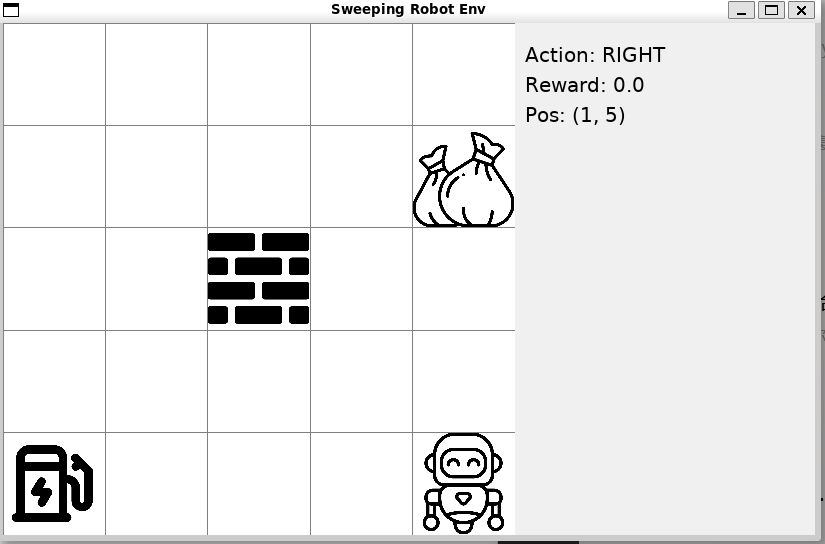
\includegraphics[width=0.48\linewidth]{figure/sweep_robot_env_render1.jpg}
% \hfill
% 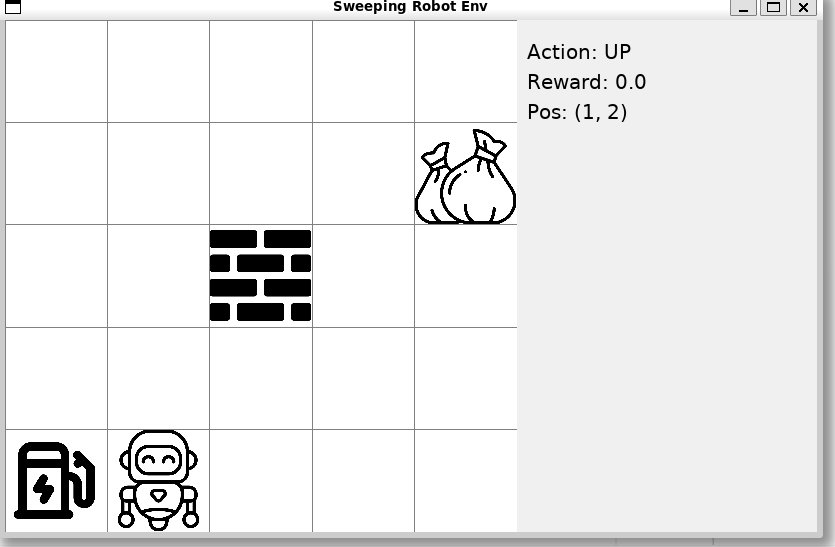
\includegraphics[width=0.48\linewidth]{figure/sweep_robot_env_render2.jpg}
% \caption{扫地机器人学习过程可视化展示(\textsf{render} 函数实现)}\label{fig:sweeping-robot-env-render}
% \end{figure}

\begin{figure}[htb]
\centering
\begin{subfigure}{0.48\linewidth}
    \centering
    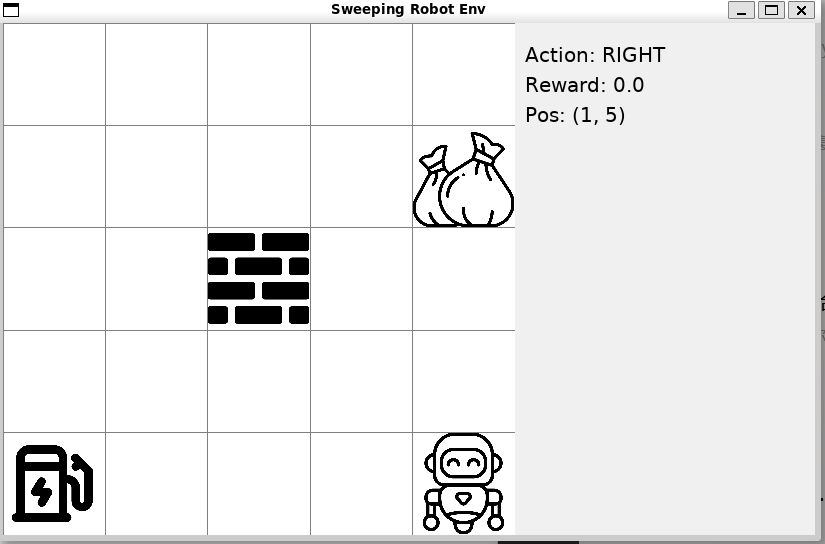
\includegraphics[width=\linewidth]{figure/sweep_robot_env_render1.jpg}
\end{subfigure}
\hfill
\begin{subfigure}{0.48\linewidth}
    \centering
    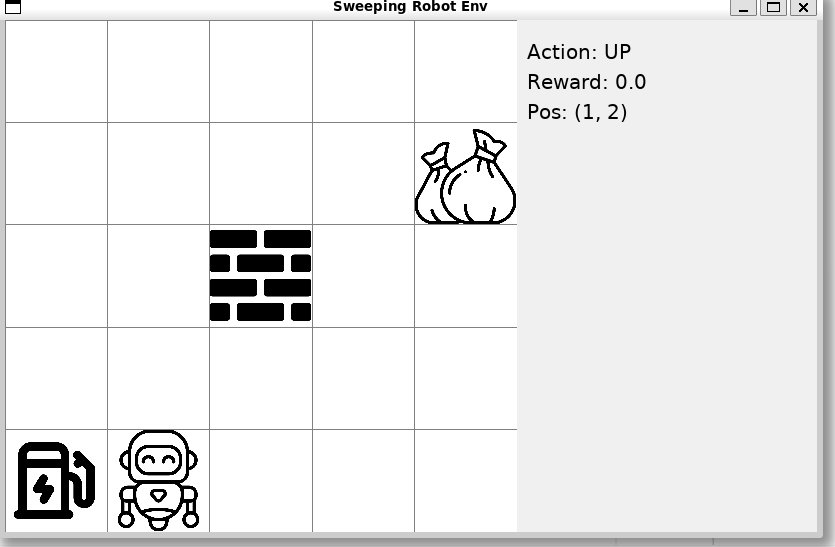
\includegraphics[width=\linewidth]{figure/sweep_robot_env_render2.jpg}
\end{subfigure}
\caption{扫地机器人学习过程可视化展示(\textsf{render} 函数实现)}
\label{fig:sweeping-robot-env-render}
\end{figure}

\subsection{具体代码}

对于扫地机器人的环境的具体代码,请参考附录~\ref{sec:sweeping-robot-env}